\documentclass[tikz]{standalone}

\begin{document}
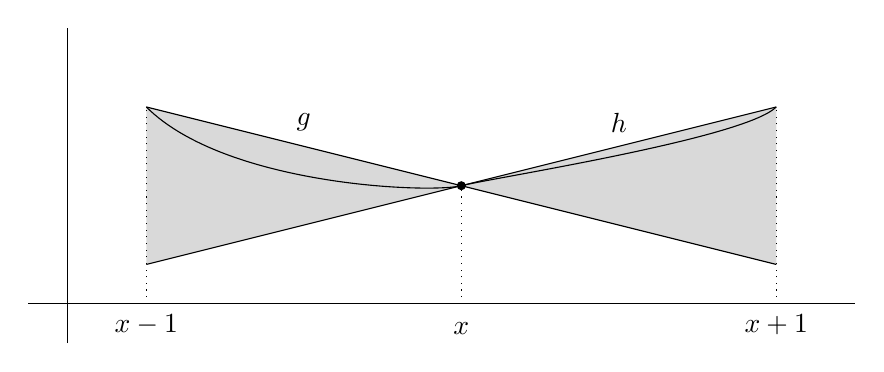
\begin{tikzpicture}[scale=2]
  \draw (-0.5, -0.5) -- (-0.5, 1.5);
  \draw (-0.75, -0.25) -- (4.5, -0.25);
  \fill[black!15] (0, 1) -- (2, 0.5) -- (0, 0) -- cycle;
  \fill[black!15] (4, 1) -- (2, 0.5) -- (4, 0) -- cycle;
  \draw (0, 1) .. controls +(0.5, -0.5) and +(-0.2, -0.05)
    .. (2, 0.5) .. controls +(0.2, 0.05) and +(-0.2, -0.2)
    .. (4, 1);
  \draw[fill=black] (2, 0.5) circle (0.025);
  \draw (4, 1) -- (0, 0);
  \draw (0, 1) -- (4, 0);

  \draw[dotted] (0, -0.25) -- (0, 1);
  \draw[dotted] (2, -0.25) -- (2, 0.5);
  \draw[dotted] (4, -0.25) -- (4, 1);

  \node at (0, -0.38) {$x-1$};
  \node at (2, -0.41) {$x$};
  \node at (4, -0.38) {$x+1$};

  \node at (3, 0.9) {$h$};
  \node at (1, 0.9) {$g$};
\end{tikzpicture}
\end{document}
